\documentclass{notes}
\usepackage[makeroom]{cancel}

\author{Ritchie Cai, Matthew Mosley \& Corey Higgins}
\title{Inverted Pendulumn Modeling}

\begin{document}
\maketitle 

\section{Description}
Our design project is to simulate and implement a inverted pendulum using 
$\text{Lego Mindstorm EV3}^{\textregistered}$. 

\section{Physical Model}

Our goal is to balance a two wheeled inverted pendulum. The pendulum setup is shown in 
figure~\ref{fig:lego_build}.

\begin{figure}[t]
  \begin{minipage}[b]{2.5in}
    \centerline{\mbox{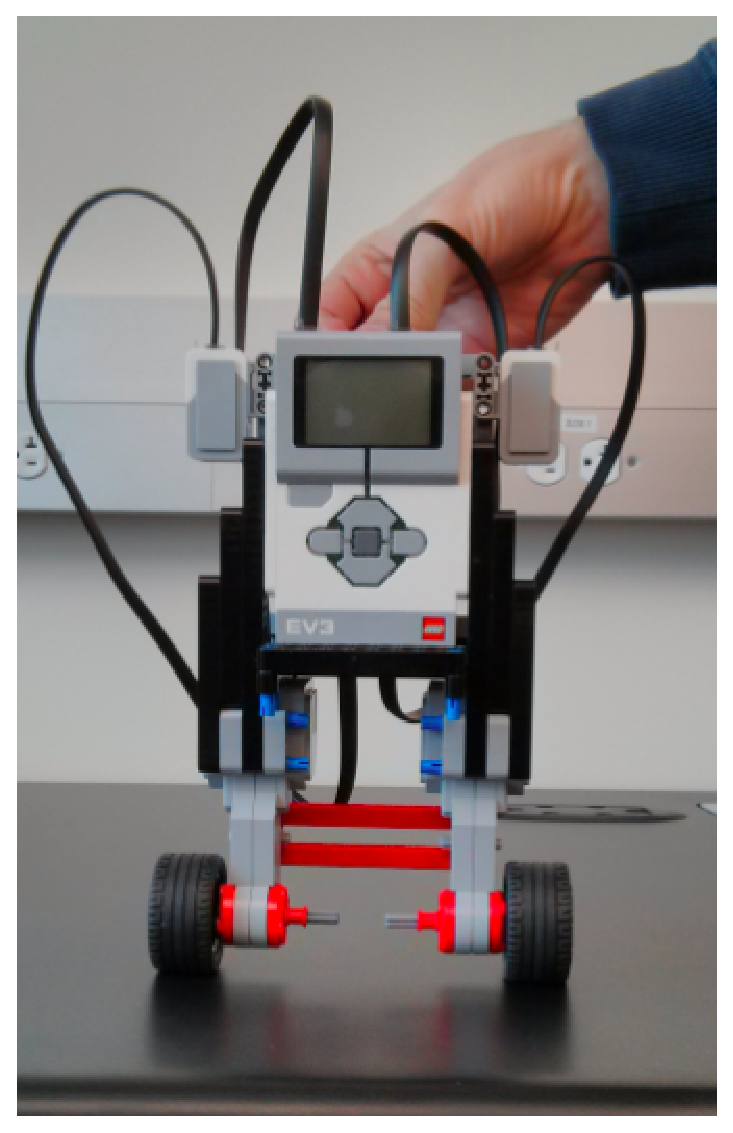
\includegraphics[width=2.5in]{pics/Lego/Build_front.eps}}}
    \centerline{\emph{(a) front view}}
  \end{minipage}
  \begin{minipage}[b]{2.5in}
    \centerline{\mbox{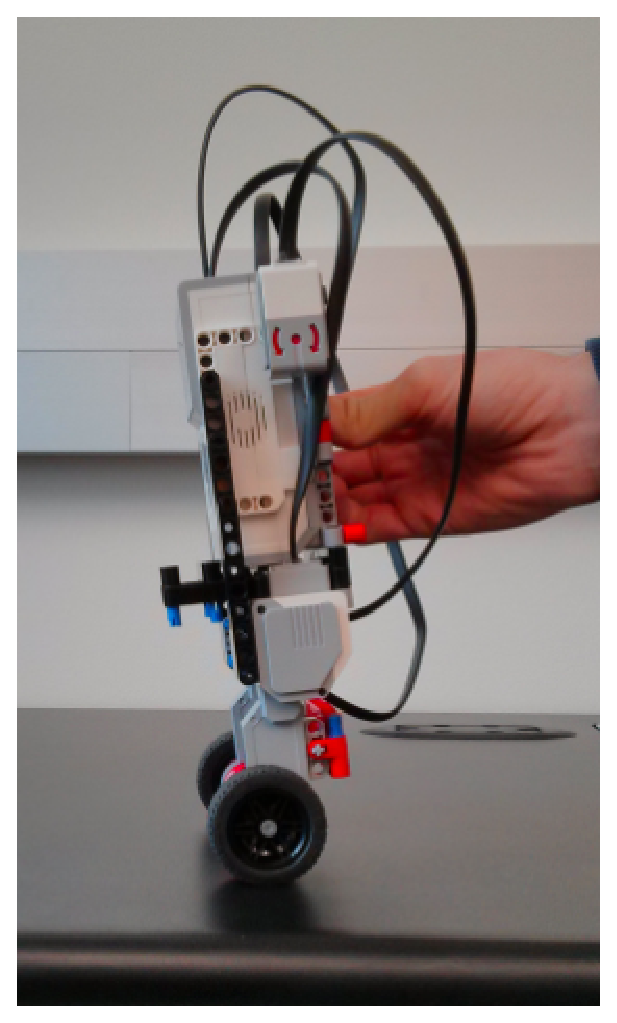
\includegraphics[width=2.5in]{pics/Lego/Build_side.eps}}}
    \centerline{\emph{(b) side view}}
  \end{minipage}
  \caption{Lego two wheeled inverted pendulum setup}
  \label{fig:lego_build}
\end{figure}

On the top of the pendulum, there are two gyro sensors, one on each side. the actual angle of the
pendulum body will be measured by averaging the two readings from gyro sensors. The bottom of the
pendulum is controlled by two motors. Motors can be controlled in terms of number of rotations,
angular volecity and angular acceleration.

% The rod on top of the cart can only lean forward and backward. 
% Base cart also can move only move back and forth. 
% When the rod is out of balance and leaning toward one side, the cart will accelerate toward the same
% direction to make sure the rod is back to resting position relative to the cart.

% \begin{figure}[!h]
%   \begin{center}
%     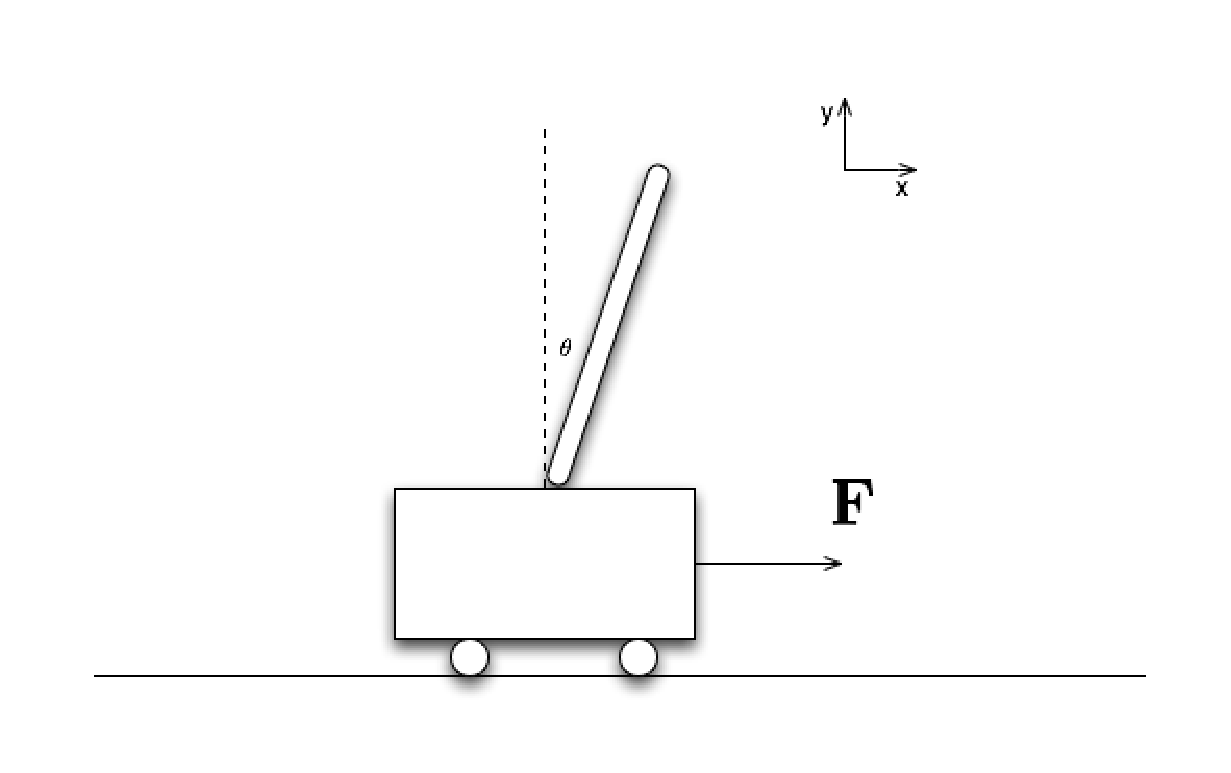
\includegraphics[width=3.5in]{pics/full_system.eps}
%   \end{center}
%   \caption{System setup for inverted pendulum}
%   \label{fig:full_system}
% \end{figure}


\section{Mathematical Model}

For simplicity, the body of two wheeled inverted pendulum is modeld as a straight rod with evenly
distributed mass. So the center the mass should be in the middle of the rod. We analyze the system
from two perspective, one from x-axis and one form y-axis. Then combining them together. Symbols we
used in the derivation is defined as follows: 
\begin{description}
  \item[$M$]{Mass of the two wheels.}
  \item[$m$]{Mass of the pendulum body.}
  \item[$L$]{Length of our pendulum.}
  \item[$x$]{Position of the system on x-axis}
  \item[$y$]{Position of the system on y-axis}
  \item[$a_t$]{Tangential acceleration.}
  \item[$a_c$]{Centripetal acceleration.}
  \item[$\theta$]{Angle of the pendulum.}
  \item[$\omega$]{Angluar volecity of the wheels}
\end{description}

\subsection{X-axis}
On the horizontal, x-axis, we have:

\begin{align*}
  % F_x & = F_{cart} + F_{rod} \\
  % F_{cart} & = M\ddot{x}  \\
  % F_{rod}  & = m a_x + m a_{p} \\
  %         & = m \ddot{x} + m (a_{t} + a_{c})
  F_x = 	M\frac{L}{2}\ddot{x}\cos{\theta}
  		+\frac{mL}{2}\ddot{x}\cos{\theta}
  		-m\left(\frac{L}{2}\right)^2\ddot{\theta}\cos^2{\theta}
		-m\left(\frac{L}{2}\right)^2\dot{\theta}^2\sin{\theta}\cos{\theta}
\end{align*}

%where $a_t$ and $a_c$ are tangential and centripetal acceleration respectively. 

\begin{figure}[!h]
  \begin{center}
    \begin{minipage}[b]{3.5in}
      \centerline{\mbox{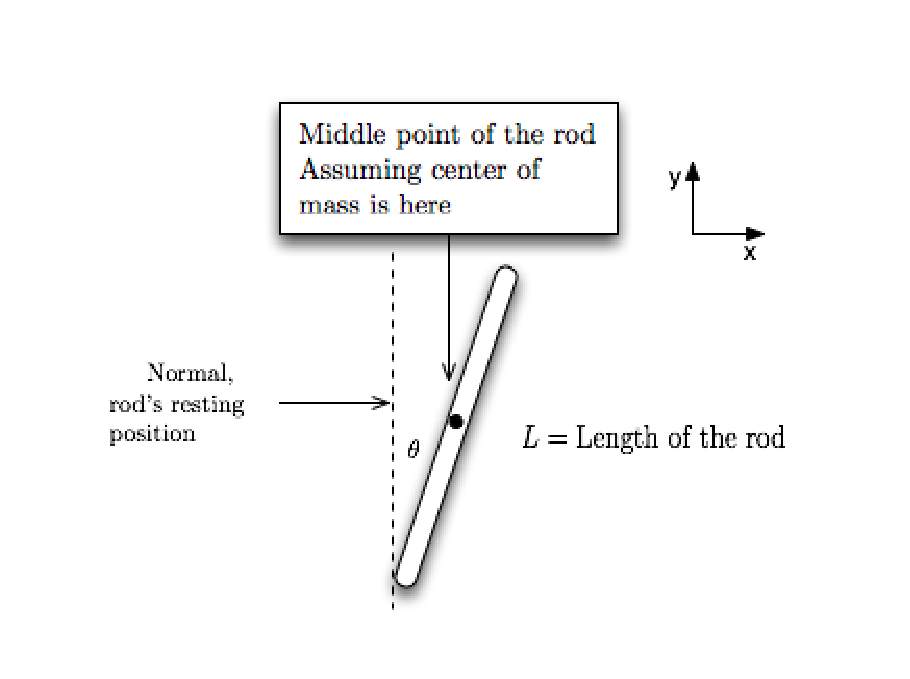
\includegraphics[width=3.5in]{pics/rod.eps}}}
    \end{minipage}
    \begin{minipage}[b]{3.5in}
      \centerline{\mbox{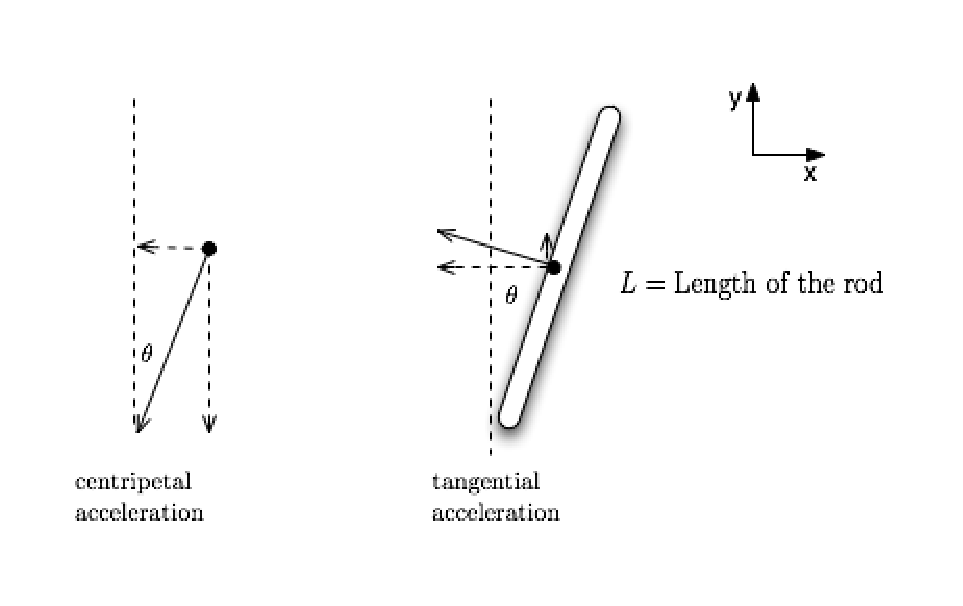
\includegraphics[width=3.5in]{pics/rod_acceleration.eps}}}
    \end{minipage}
    
  \end{center}
  \caption{Angular acceleration disection for the rod}
  \label{fig:angular_rod}
\end{figure}

According to figure~\ref{fig:angular_rod}, angular accelerations for the rod on x-axis can be
expressed as:
\begin{align*}
  a_t & = -\dfrac{L}{2} \ddot{\theta} \\
  a_c & = -\dfrac{L}{2} \dot{\theta}^2
\end{align*}

Since we are only interested in the components on the x-axis, we have:

\begin{align*}
  a_t & = -\dfrac{L}{2} \ddot{\theta} \cos \theta \\
  a_c & = -\dfrac{L}{2} \dot{\theta}^2 \sin \theta
\end{align*}

So 

\begin{align}
  F_x  & = m \ddot{x} + m (a_{t} + a_{c}) \nonumber\\
         & = m \ddot{x} -m\dfrac{L}{2} \ddot{\theta} \cos \theta 
                        -m\dfrac{L}{2} \dot{\theta}^2 \sin \theta \label{eqn:f_x}
      % & = (M + m) \ddot{x} - m\dfrac{L}{2} \ddot{\theta} \cos \theta 
      %               - m \dfrac{L}{2} \dot{\theta}^2 \sin \theta \label{eqn:f_x}
\end{align}
\FloatBarrier


\subsection{Y-axis}
Using Newton's second law for the vertical motion of the pendulum gives

\begin{align*}
  % F_y & = ma_y - mg \label{eqn:eq1} \\
  F_y & = ma_y - mg \\
      & = m(a_t + a_c) - mg
\end{align*}
where $a_y$, $a_t$ and $a_c$ are acceleration of y-axis, tangential and centripetal of the rotation
respectively. 

Using figure~\ref{fig:angular_rod}, we can express the acceleration on y-axis with:
\begin{align*}
  a_t & = \dfrac{L}{2}\ddot{\theta}\sin\theta \\
  a_c & = -\dfrac{L}{2}\dot{\theta}^2\cos\theta
\end{align*}

So

\begin{align}
  F_y & = m(a_t + a_c) - mg \nonumber\\
      & = m(\dfrac{L}{2}\ddot{\theta}\sin\theta - \dfrac{L}{2}\dot{\theta}^2\cos\theta) - mg
      \nonumber\\ 
      & = m\dfrac{L}{2}\ddot{\theta}\sin\theta - m\dfrac{L}{2}\dot{\theta}^2\cos\theta - mg
       \label{eqn:f_y}
\end{align}

 % Since $ y = \dfrac{L}{2}\cos\theta$,

 % \begin{align}
 %   \dot{y} & = \frac{d(l/2\cos\theta)}{dt} = -\dfrac{L}{2}\ddot{\theta}\sin\theta \nonumber\\
 %   % \frac{dy_G}{dt} & = \frac{d(l/2\cos\theta)}{dt} = -l/2\sin\theta\frac{d\theta}{dt} \nonumber\\
 %   \frac{d^2y_G}{dt^2} & = \frac{d}{dt}\left(-l/2/2 \sin\theta \frac{d\theta}{dt}\right) \nonumber\\
 %   & = -l/2/2\left(\frac{d\sin\theta}{dt}\frac{d\theta}{dt} + \sin\theta\frac{d^2\theta}{dt^2}\right) \nonumber\\
 %   & = -l/2\left( \cos\theta \left(\frac{d\theta}{dt}\right)^2 + \sin\theta\frac{d^2\theta}{dt^2}   \right) \nonumber\\
 %   & = -l/2\cos\theta\left(\frac{d\theta}{dt}\right)^2-l/2\sin\theta\frac{d^2\theta}{dt^2}\label{eqn:eq2}
 % \end{align}
 
 % Using Equation~\ref{eqn:eq2}, Equation~\ref{eqn:eq1} can be written as 
 % \begin{align*}
 %   F_y - mg & = m(-\frac{L}{2}\dot{\theta}^2\cos\theta - \frac{L}{2}\ddot{\theta}\sin\theta )
 % \end{align*}
 
 % Thus, the vertical reaction force, $F_y$, can be written as
 % \begin{align*}
 %   F_y & = mg + m\left(-\frac{L}{2}\dot{\theta}^2\cos\theta - \frac{L}{2}\ddot{\theta}\sin\theta\right)
 % \end{align*}

 \subsection{Angular Momentum}
 
 For any object, the relationship between the moment applied on an object and its angular acceleration is given by the following relationship
 \begin{align}
   I \ddot{\theta} = \sum \overline{M} \label{eqn:torque}
 \end{align}
 
 where $\overline{M}$ is the moment due to a given force and defined as 
 
 \[
 \overline{M} = \vec{F} \times \vec{r}
 \]
 
 where $\vec{F}$ is the force vector, $\vec{r}$ is the position vector of the object with respect to
 the point about which the moments are being summed, and $I$ is the angular momentum of the object.
 For the pendulum, summing the moment around the center of gravity, Equation~\ref{eqn:torque} can be
 written as

 \begin{eqnarray*}
   I\ddot{\theta} & = & F_y\dfrac{L}{2}\sin\theta - F_x\dfrac{L}{2}\cos\theta \\
     & = & \left( m\dfrac{L}{2}\ddot{\theta}\sin\theta - m\dfrac{L}{2}\dot{\theta}^2\cos\theta 
            - mg\right) \dfrac{L}{2}\sin\theta \\
     &   & -\left( m\ddot{x} - m\dfrac{L}{2}\ddot{\theta}\cos\theta - 
             m\dfrac{L}{2}\dot{\theta}^2\sin\theta \right) \dfrac{L}{2}\cos\theta\\
     & = & m\dfrac{L^2}{4}\ddot{\theta}\sin^2\theta 
           - \cancel{m\dfrac{L^2}{4}\dot{\theta}^2\cos\theta\sin\theta} - \dfrac{L}{2}mg\sin\theta\\
     &   & - m \dfrac{L}{2} \ddot{x}\cos\theta + m\dfrac{L^2}{4}\ddot{\theta}\cos^2\theta + 
             \cancel{m\dfrac{L^2}{4}\dot{\theta}^2\sin\theta\cos\theta} \\
     & = & m\dfrac{L^2}{4}\ddot{\theta}\cancelto{1}{(\sin^2\theta + \cos^2\theta)}
           - \dfrac{L}{2}mg\sin\theta - m \dfrac{L}{2}\ddot{x}\cos\theta \\
     & = & m \dfrac{L^2}{4}\ddot{\theta} - \dfrac{L}{2}mg\sin\theta 
           - m \dfrac{L}{2} \ddot{x}\cos\theta
    %               & = & (mg 
    %                    + m(-l\ddot{\theta}\cos\theta - l\ddot{\theta}\sin\theta)
    %                   )l\sin\theta 
    %                   -m(\ddot{x} 
    %                       - \ddot{\theta}l\sin\theta + \ddot{\theta}l\cos\theta
    %                   )l\cos\theta \\
    % & = & mgl\sin\theta - ml^2\ddot{\theta}\cos\theta\sin\theta- ml^2\ddot{\theta}\sin^2\theta \\
    % &  & - ml\ddot{x}\cos\theta + ml^2\ddot{\theta}\cos\theta\sin\theta 
    %     - ml^2\ddot{\theta}\cos^2\theta \\
    % & = & mgl\sin\theta - ml^2\ddot{\theta}(\sin^2\theta + \cos^2\theta) - ml\ddot{x}\cos\theta \\
    % & = & mgl\sin\theta - ml^2\ddot{\theta} - ml\ddot{x}\cos\theta 
 \end{eqnarray*}

We are assuming the center of gravity and the center of mass of the rod are at the same point, so
there is no angular movement of the rod around it's center. Therefore:

\begin{align}
  I\ddot{\theta} & = 0 \nonumber\\
  m \dfrac{L^2}{4}\ddot{\theta} - \dfrac{L}{2}mg\sin\theta 
      - m \dfrac{L}{2} \ddot{x}\cos\theta  & = 0 \nonumber\\
  \dfrac{L}{2}\ddot{\theta} - g\sin\theta - \ddot{x}\cos\theta & = 0 \nonumber
\end{align}

Using linear approximation, we approximate:

\begin{align}
  \dfrac{L}{2}\ddot{\theta} - g\theta - \ddot{x} & = 0 \label{eqn:pre_tf} \\ 
  & \begin{cases}
    \sin\theta \approx \theta \nonumber\\
    \cos\theta \approx 1\nonumber\\
  \end{cases}
\end{align}
 
\noindent Taking Laplace transform of equation~\ref{eqn:pre_tf}, we have: 

\begin{align*}
  \dfrac{L}{2}s^2\Theta - g\Theta & = U \\
  \Theta & = \dfrac{\frac{2}{L}}{s^2 - \frac{2g}{L}}U
\end{align*}
where $U$ is an input acceleration (replacing $\ddot{x}$)\\

\noindent We now have the following transfer function:

\[
  T(s) = \dfrac{\Theta}{U} = \dfrac{\frac{2}{L}}{s^2-\frac{2g}{L}}
\]

\begin{figure}[!h]
  \begin{center}
    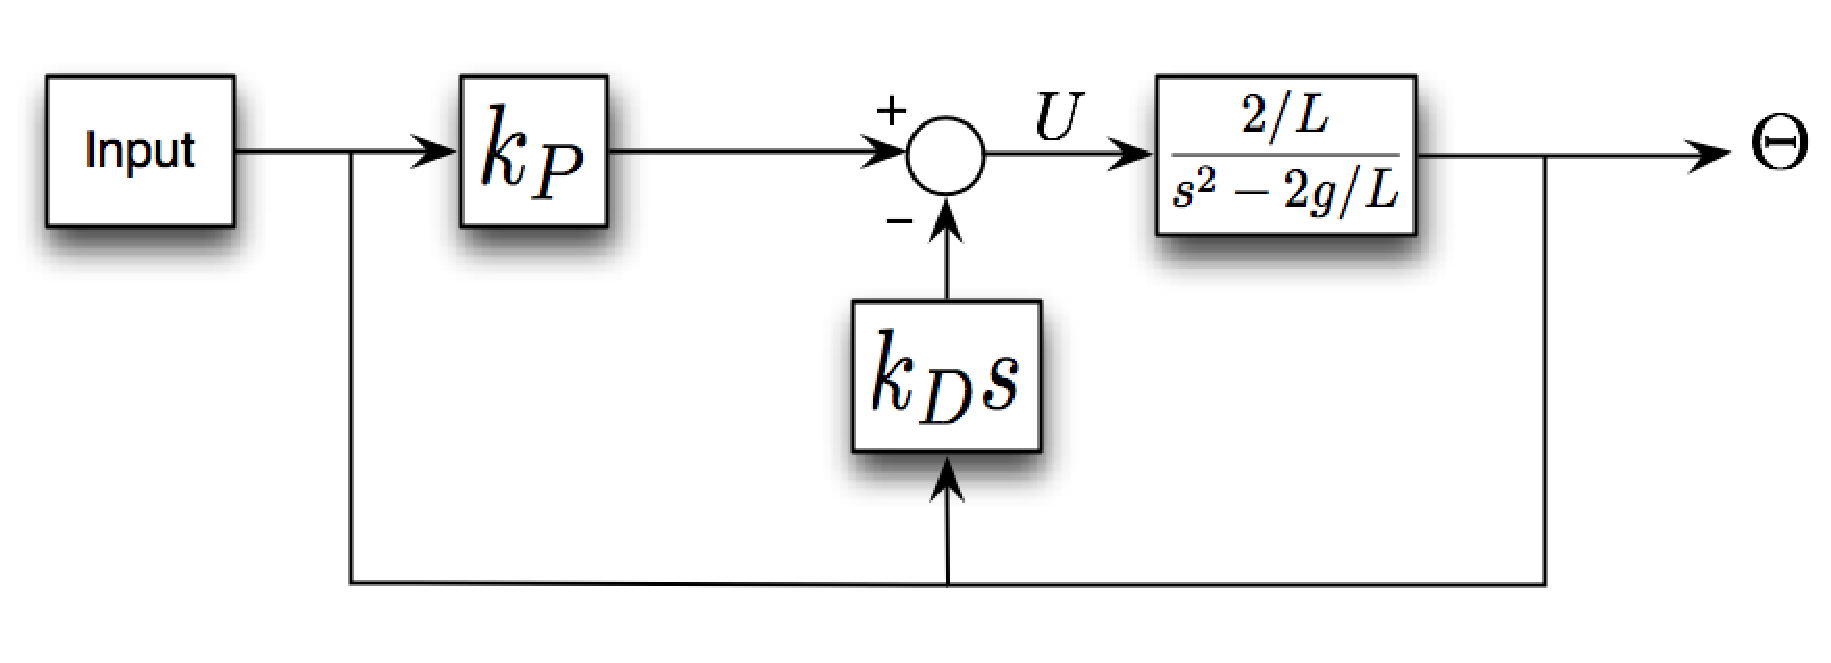
\includegraphics[width=4.5 in]{pics/tf.eps}
  \end{center}
  \caption{Block diagram for our system}
  \label{fig:block_diagram}
\end{figure}

We will use the  techniques we have learned this semester to find appropriate values for $k_P$ and $k_D$ to ensure system stability. We have yet to determine the input signal to be controlled in Figure~\ref{fig:block_diagram}.

\newpage
\section{Performance Measurements}
The settling time was found to be 1.22 seconds. 



\end{document}
